\documentclass[11pt]{article}
\usepackage{graphicx}
\usepackage{fullpage}
\usepackage{anysize}
\usepackage{caption}
\usepackage{titlesec}
\usepackage[usenames,dvipsnames, x11names]{xcolor} % load xcolor and make it recognise the names... 
\usepackage{colortbl}
\usepackage{color, soul} %the soul package allows you to hilight text with \hl{}
\usepackage{hyperref}   % this creates hyperlinks for figure and table referencing (and all other referencing too!)
\usepackage{csvsimple}
\usepackage{tablefootnote}
\usepackage{floatrow}  % to hepl place table captions
\usepackage[hang,flushmargin]{footmisc} %The 'hang' option flushes the footnote marker to the left margin of the page, while the 'flushmargin' option flushes the text as well
\usepackage{lipsum} % these two are required to get good table footnotes
\usepackage{threeparttable}
\usepackage{tikz}
\usepackage{longtable}
\usepackage{gensymb}
%%%%%%%%%%%%%%%%%%%%%%%%%
% Defining format for hyperlinks 
\hypersetup{colorlinks, % left blank (no == to) so no red square
linkcolor= PineGreen, 
filecolor= TealBlue, 
urlcolor= PineGreen,
citecolor= NavyBlue}
\RequirePackage[margin=1in]{geometry} % customize margins 
\RequirePackage{pdflscape}
% this bit sets the section formatting
\titleformat{\section}
  {\normalfont\sffamily\Large\bfseries\color{CornflowerBlue}}
  {\thesection}{1em}{}
% this bit sets the caption formatting formatting
\usepackage[font={bf,small}]{caption}
% to get the table captions at the top of the table
\floatsetup[table]{capposition=top}
% remove the paragraph indenting 
%\setlength{\parindent}{0pt}
\setlength{\parskip}{1em}
\newcommand{\spper}{\hspace{0.5mm}\%}
\newcommand{\spkg}{\hspace{0.5mm}kg}
\newcommand{\spmt}{\hspace{0.5mm}mt}

%________________________________________________
% Change this to the path of the individual country
% \newcommand{\CntPath}{C:/Longline_Reports/Plots/TO}
% \newcommand{\GenPath}{C:/Longline_Reports/Plots}
% \newcommand{\CntLb}{TO}
%________________________________________________


\usepackage{Sweave}
\begin{document}
\Sconcordance{concordance:WHATapp_Report.tex:WHATapp_Report.Rnw:%
1 51 1 1 0 3 1 1 7 292 1}


% grab my numbers and tables created in R

% make the cover page
\pagenumbering{gobble} % switch off page numbering
\makeatletter
\def\parsecomma#1,#2\endparsecomma{\def\page@x{#1}\def\page@y{#2}}
\tikzdeclarecoordinatesystem{page}{
    \parsecomma#1\endparsecomma
    \pgfpointanchor{current page}{north east}
    % Save the upper right corner
    \pgf@xc=\pgf@x%
    \pgf@yc=\pgf@y%
    % save the lower left corner
    \pgfpointanchor{current page}{south west}
    \pgf@xb=\pgf@x%
    \pgf@yb=\pgf@y%
    % Transform to the correct placement
    \pgfmathparse{(\pgf@xc-\pgf@xb)/2.*\page@x+(\pgf@xc+\pgf@xb)/2.}
    \expandafter\pgf@x\expandafter=\pgfmathresult pt
    \pgfmathparse{(\pgf@yc-\pgf@yb)/2.*\page@y+(\pgf@yc+\pgf@yb)/2.}
    \expandafter\pgf@y\expandafter=\pgfmathresult pt
}
\makeatother

\begin{tikzpicture} [remember picture, overlay,every node/.style={anchor=center}] {               
\node  at (page cs:0,0.8) {                                % [anchor=\bound]

\includegraphics [width=22cm]{C:/GitHub/WHATapp/Writing/flag_logos/banner_new.png}};
\node  at (page cs:0,0.3) [blue]{ 
{{\huge{\bfseries An introduction to the WHATapp tool for}}}};
\node  at (page cs:0,0.23) [blue]{ 
{{\huge{\bfseries visualising high seas allocations}}}};
\node  at (page cs:0,-0.05) {

\includegraphics [width= 3in]{C:/GitHub/WHATapp/Writing/flag_logos/FFA.png}};
\node  at (page cs:0,-0.6) {

\includegraphics [width= 1in]{C:/GitHub/WHATapp/Writing/flag_logos/NZ_aid_logo.png}};
\node  at (page cs:0,-0.4) {
{\Large This work was funded by the New Zealand Aid Progamme.}};
\node  at (page cs:0,-0.8) [blue]{ 
{Issue Specific National Report, (An introduction to WHATapp for visualising allocations) October 2019 }};
\node  at (page cs:0,-0.85) [blue]{ 
{\small Please address inquiries to: Sam McKechnie (samm@spc.int)  }};
\draw [thick] [blue] (page cs:-1,-0.75) rectangle (page cs:1,-0.75);
     }
\end{tikzpicture}
\clearpage     % goes to new page but progresses all floating figures up to that point 
%\restoregeometry

\pagenumbering{arabic}  % start the page numbering again
\section{Introduction} \label{sec:intro}
The establishment of hard limits and allocations for the high seas were addressed in CMM 2017-01 with decisions about the process of allocating high seas fishing being scheduled for the 2019 commission meeting. In preparation, FFA members have conducted a series of workshops to develop criteria and a strategy for approaching the allocation process. These have highlighted the complexity of the issues involved, the large number of potential criteria that may be considered, the diverse approaches taken by other tuna RFMOs and similar bodies, and the potentially conflicting rankings that various CCMs in the WCPFC will give to different criteria.

Although there are difficulties in identifying (and sometimes formulating) criteria, what is clear is the need for members to have a means of visualising allocations under different scenarios. This is particularly the case when allocations are based on multiple criteria, each of which may be given different weightings. Initial tools to this end were constructed in excel and have recently been extended to ``Shiny'' - software based on the R statistical language that allows the construction of interactive web-based applications (apps). This report is intended to be a support document that demonstrates how to install and run the app, the range of features that can be modified, and explicitly outlines the calculations behind the scenarios included.

The app is simply a tool to visualise the criteria (and their weightings) and so the difficulties associated with the allocation process tend to be centred around the selection and formulation of the criteria, rather than the development of the app itself. For example, some criteria such as economic dependency are difficult to define and synthesise into discrete values for each CCM. The set of criteria included in the app and the methods to weight them should not therefore be considered a final set or an accepted methodology. We will continue to develop the app to suit the needs of the membership as further criteria are suggested or existing criteria are modified.

\section{Running the app}
Shiny apps are typically run either via a local server which requires users to have the R software (and applicable packages) installed, or are web-based which requires a robust internet connection. These are both barriers to easy distribution of an app, for example at workshops - particularly in the Pacific where internet connectivity can be limited.

We have therefore developed a fully portable version of the app that does not require internet access, or the installation of R and knowledge of its use. The downside of this approach is that a web browser and a portable version of R must be packaged together with the usual components of the app. This leads to a relatively large file size, although  no true ``installation'' is necessary and so deletion of the app after use is simple. At this stage it is also restricted to windows operating systems. 

The first step in using the app is to download the zipped file from the web or copy it from an external harddrive. This should be unzipped to where you want to store and run the app from. It is recommended to unzip the file to somewhere other than the ``downloads'' folder as it may be difficult to run the executable from this location. Now click into the WHATapp folder and you should see a file structure very similar to that shown in Fig. \ref{fig:expl1screen}. Running the app is a simple matter of double clicking on run.bat (one of the options circled in Fig. \ref{fig:expl1screen}). Note that you must not only close the app window but also close the black command prompt window (Fig. \ref{fig:batscreen}) to completely terminate the app after you have finished using it.

%Running the app is a simple matter of double clicking run.vbs as a first choice, or alternatively run.bat (both circled in Fig. \ref{fig:expl1screen}). Note that if utilising the run.bat option you must not only close the app window but also close the black command prompt window (Fig. \ref{fig:batscreen}) to completely terminate the app after you have finished using it.

Depending on the security settings on your machine you may encounter a warning popup window the first time you double click the run.vbs or run.bat. {\bf Click XXXX.}. Alternatively, try right clicking the run.vbs or run.bat and selecting ``Run as administrator''. With any luck the app will successfully launch after a few seconds and you should see a screen similar to Fig. \ref{fig:frontpg}. If the formatting of the browser window is messy then it should be possible to adjust this by zooming in (press ``ctrl'' and ``+'') or out (press ``ctrl'' and ``-'').

 \begin{figure} [h]
  \centering
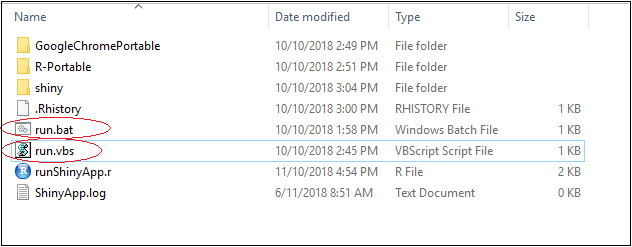
\includegraphics[width=1\textwidth]{C:/GitHub/WHATapp/Writing/Explorer_Folder_1.png}
  \caption {The layout of the WHATapp folder that should be unzipped onto your machine. Click ``run.bat'' to launch the application.}
  \label{fig:expl1screen}
\end{figure}


 \begin{figure} [h]
  \centering
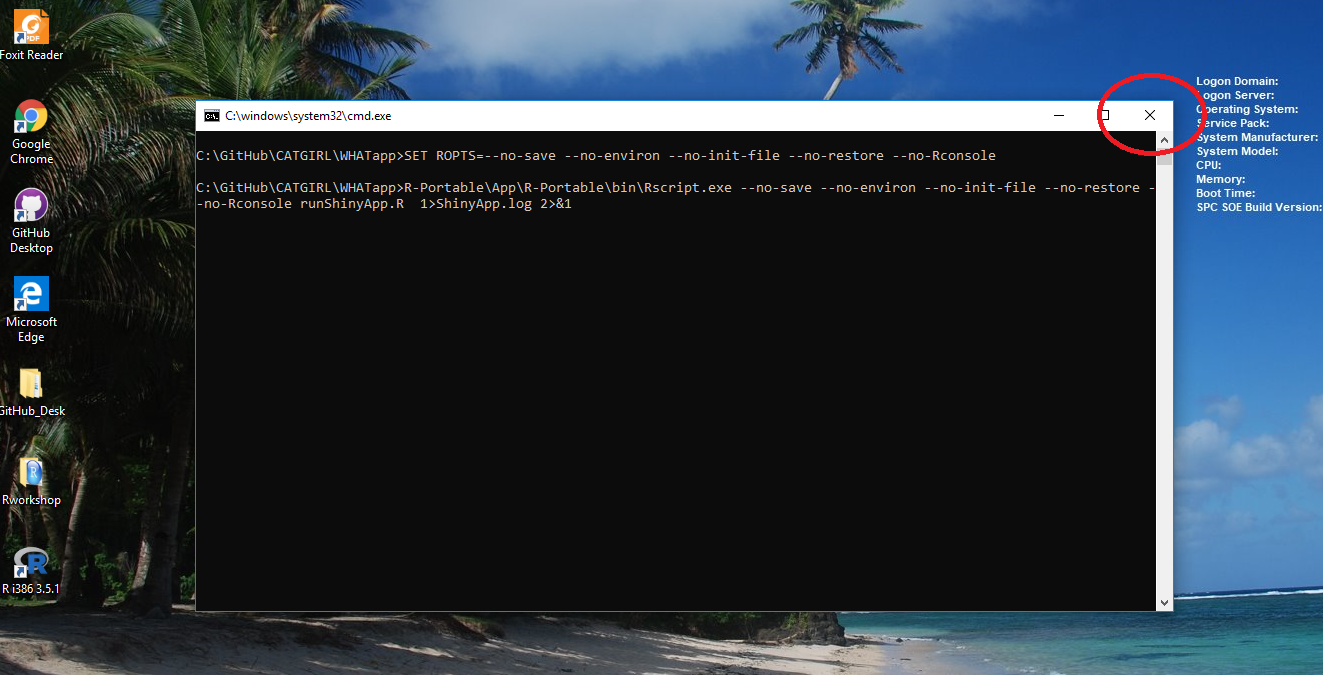
\includegraphics[width=1\textwidth]{C:/GitHub/WHATapp/Writing/Bat_Screenshot.png}
  \caption {The cmd.exe screen that must be closed when exiting WHATapp when running via the run.bat option.}
  \label{fig:batscreen}
\end{figure}


 \begin{figure} [h]
  \centering
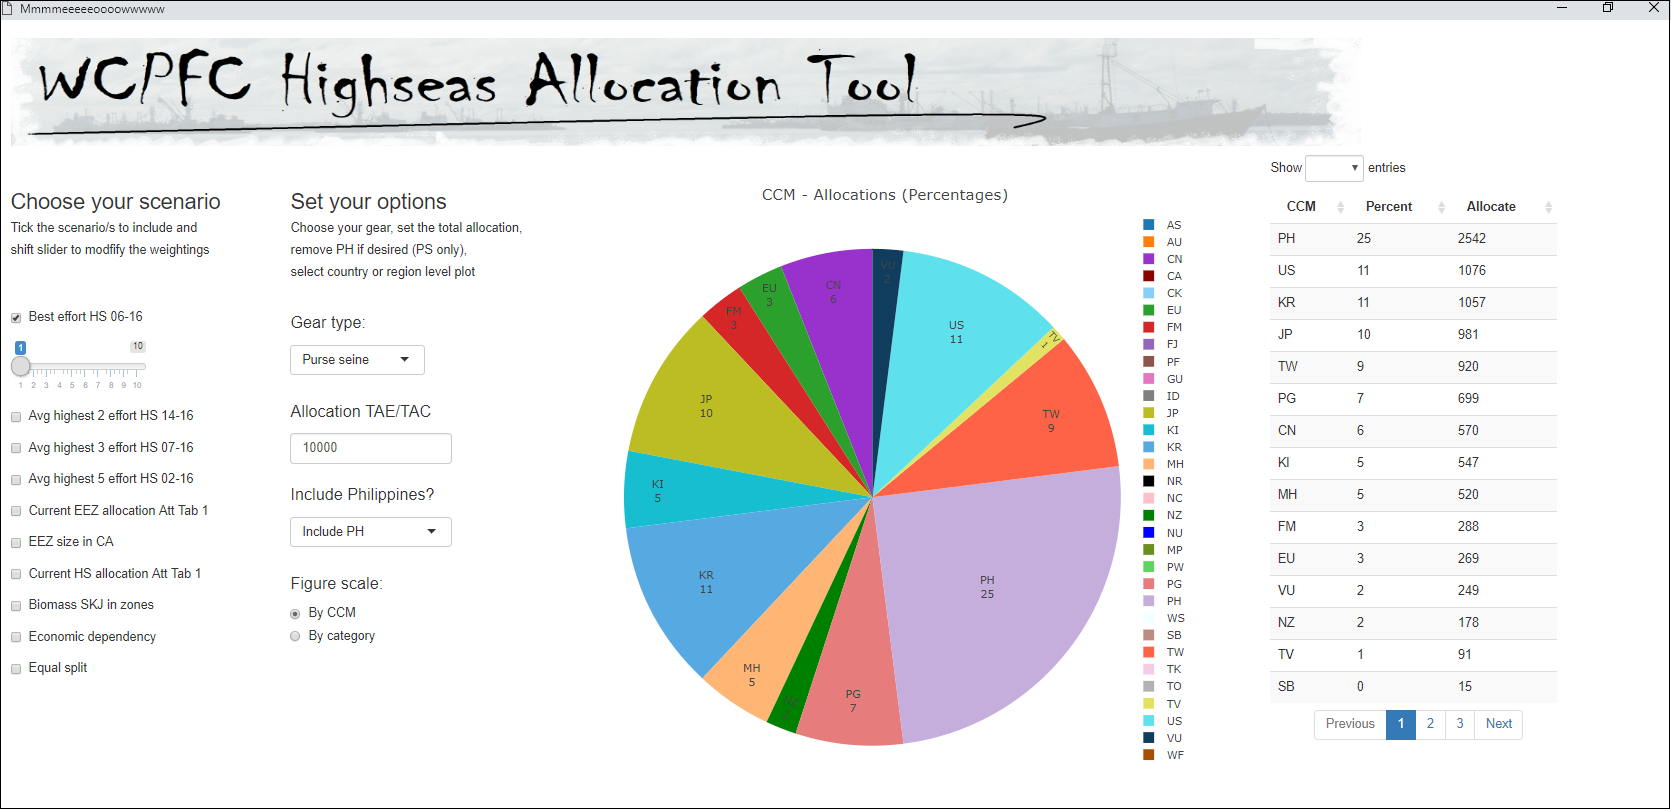
\includegraphics[width=1\textwidth]{C:/GitHub/WHATapp/Writing/App_Front_Page.png}
  \caption {A screen shot of what the browser window should look like once the application is launched. To adjust the layout of the dashboard you can zoom in and out by holding down `ctrl' and either `$+$' or `$-$'.}
  \label{fig:frontpg}
\end{figure}


 \begin{figure} [h]
  \centering
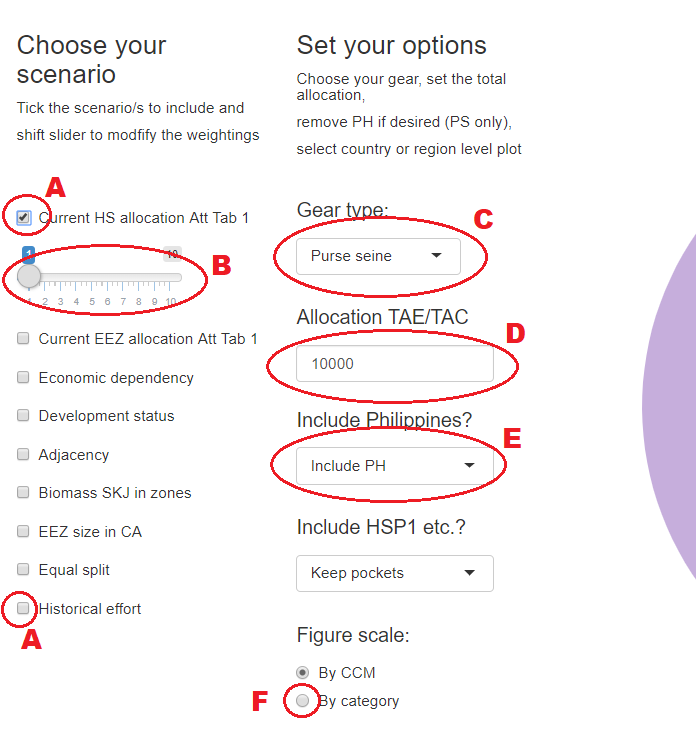
\includegraphics[width=0.8\textwidth]{C:/GitHub/WHATapp/Writing/Features_Fig.png}
  \caption {A screenshot of the application showing the control options which determine the allocation scenarios to consider (left column) and other features of the allocations that can be modified (right column).}
  \label{fig:featpg}
\end{figure}


\section{Features of the app}
\subsection{Controlling the scenarios}
Once the app is running you will see two columns of text and features on the left hand side of the dashboard (Fig. \ref{fig:featpg}). These control the scenarios that you can investigate and also some other features of the plots and tables that show the resulting allocations. To control the app you can modify the following:
\begin{itemize}
\item The left-most column (under ``Choose your scenario'') shows each of the {\bf X} criteria that can be selected and multiple scenarios can be selected simultaneously by simply clicking the appropriate check boxes (see letter {\bf A}). Further details of each scenario are presented in section \ref{sec:scendet} and the remainder of this section outlines the control of the settings.
\item Once a check box is selected and a tick appears, a slider bar will also be activated for that criteria ({\bf B}), which can be adjusted by clicking on the circle, holding the mouse button down and shifting the circle along the bar. The slider bar sets the weighting of that particular criteria with values between 1 and 10 being allowable. If only one tick box is checked then moving the slider will not impact the allocation at all (the plot and table will not change). However, if multiple boxes are ticked then the sliders determine how much weight is given to each criteria. For example, if the first two boxes are ticked and the slider for criteria 1 is set at 1, and for criteria 2 it is set at 3, then the latter will have 3 times the weighting of the former. If the slider bar for each criteria is set at 1 then they will all have the same weighting.
\item The second column of widgets defines other (than criteria) features of the app to be considered. The drop down menu ({\bf C}) allows switching between the purse seine and longline allocations. Note that there are different criteria present for the two gear types. The different gear types also have different spatial extents and these are shown in Fig. \ref{fig:HSareasPS} for both purse seine and longline.
\item The box shown by {\bf D} defines the total allowable effort (TAE; in days) and total allowable catch (TAC; in metric tonnes), for purse seine and longline respectively, from which the allocations are made. The value can be modified by clicking on the box and typing in the desired value. This number represents the total catch or effort on the high seas that must be decided before individual CCMs can be allocated specific quantities.
\item Under the purse seine scenarios there is a drop down menu that allows allocations to be made either including or excluding the Philippines (PH). The option to exclude PH is in response to the unique nature of this fleet on the high seas: they have special conditions under the CMM; are predominantly operating in high seas pocket 1; they have very low CPUE and are operationally very different from other fleets; and they have a very high effort that can dominate the effort allocations when based on historical effort criteria. For these reasons, it may be necessary for this fleet to be treated differently during allocations, and its presence in the app can obscure patterns of allocations among the remaining CCMs under certain conditions. Consequently, the user can decide if this fleet should be excluded from the visualisations or not. Note that this option does not change the allocations it simply removes PH from the visualisations to better display the allocations or the other CCMs. PH fishing in the high seas pockets can be removed entirely using the following option.
\item Also under the purse seine scenarios there is a further drop down menu that allows the user to either include or exclude several high seas pockets from the historical catch scenarios. The reason for this option is that several high seas pockets (Pockets I1, I2, I8 and I9; Fig. \ref{fig:HSfig}) were effectively closed to fishing in 2009. Including historical fishing effort in those pockets is perhaps not a desired basis for allocations based on recent fishing activity, as allocated effort may or may not be allowed in those areas. By choosing {\bf ``exclude pockets''} the allocations are calculated based on fishing effort over the remaining high seas areas in Fig.\ref{fig:HSfig}. The only other scenario that this option affects is the ``Current HS allocation Att Tab 1'' scenario which is based on the current high seas effort allocations under CMM 2018-01, which will be examined in more detail in section \ref{sec:scendet}.
\item The final option allows the user to switch between viewing the allocations by individual CCMs or by subregional groupings by clicking on the desired button. These groupings are distant water fishing nations (DWFN), FFA members that also belong to the PNA (FFA-PNA), other FFA members (FFA-OTH), Indonesia and Philippines (IDPH) and other CCMs that do not belong to any of these categories (OTH; for example New Caledonia and French Polynesia).
\end{itemize}

 \begin{figure} [h]
  \centering
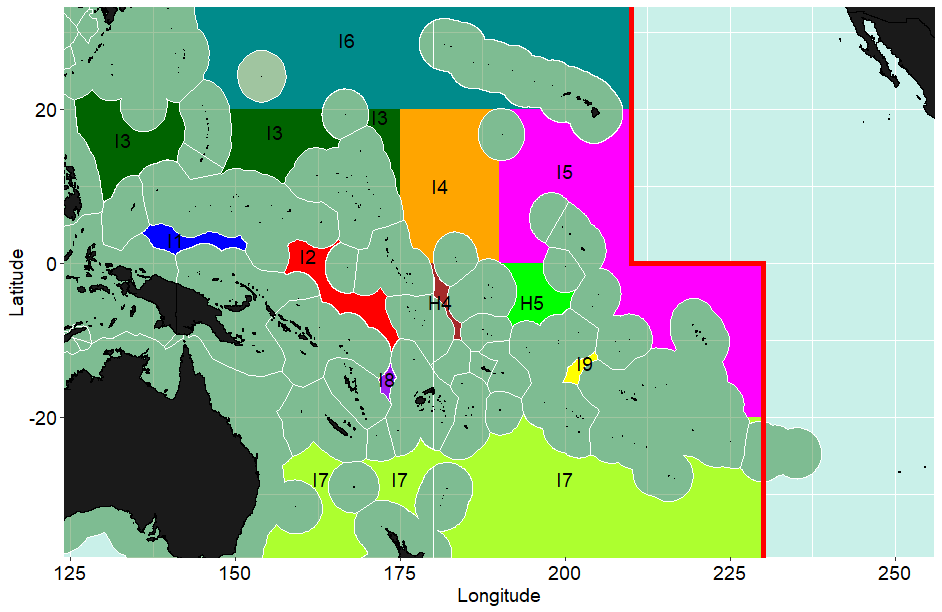
\includegraphics[width=0.95\textwidth]{C:/GitHub/WHATapp/Writing/WCPFC_HS.png}
  \caption {Map showing the high seas areas in the WCPFC and their labels, as defined by SPC.}
  \label{fig:HSfig}
\end{figure}

\subsection{Summaries of resulting allocations}
Once a certain scenario has been set and the criteria for the allocations chosen, then the app will automatically update and display the allocations for each CCM or sub regional group, with the main features illustrated in Fig. \ref{fig:outputpic}. The allocations are displayed in the form of a pie chart with the CCM/group and the proportional allocation (in percentage form - see {\bf A} in the figure) - by hovering over a pie segment the values for that CCM/group will be displayed in more detail. The chart only shows the proportional allocation and so a table is also displayed that restates the percentage allocated ({\bf B} in the figure), but also allocates the TAE/TAC into absolute allocations ({\bf C}) to the individual CCMs/groups in days (purse seine) and metric tonnes of catch (longline). Note that the format of the table is also interactive with the number of entries user-defined by the drop down box ({\bf D}) and their order can be changed by clicking on the bold table headers (e.g. ``{\bf Allocate}''; {\bf C}). If the entry in {\bf D} is left blank and not all CCMs are displayed, the ``pages'' indicated by {\bf E} can be scrolled through to find a particular CCM.

 \begin{figure} [h]
  \centering
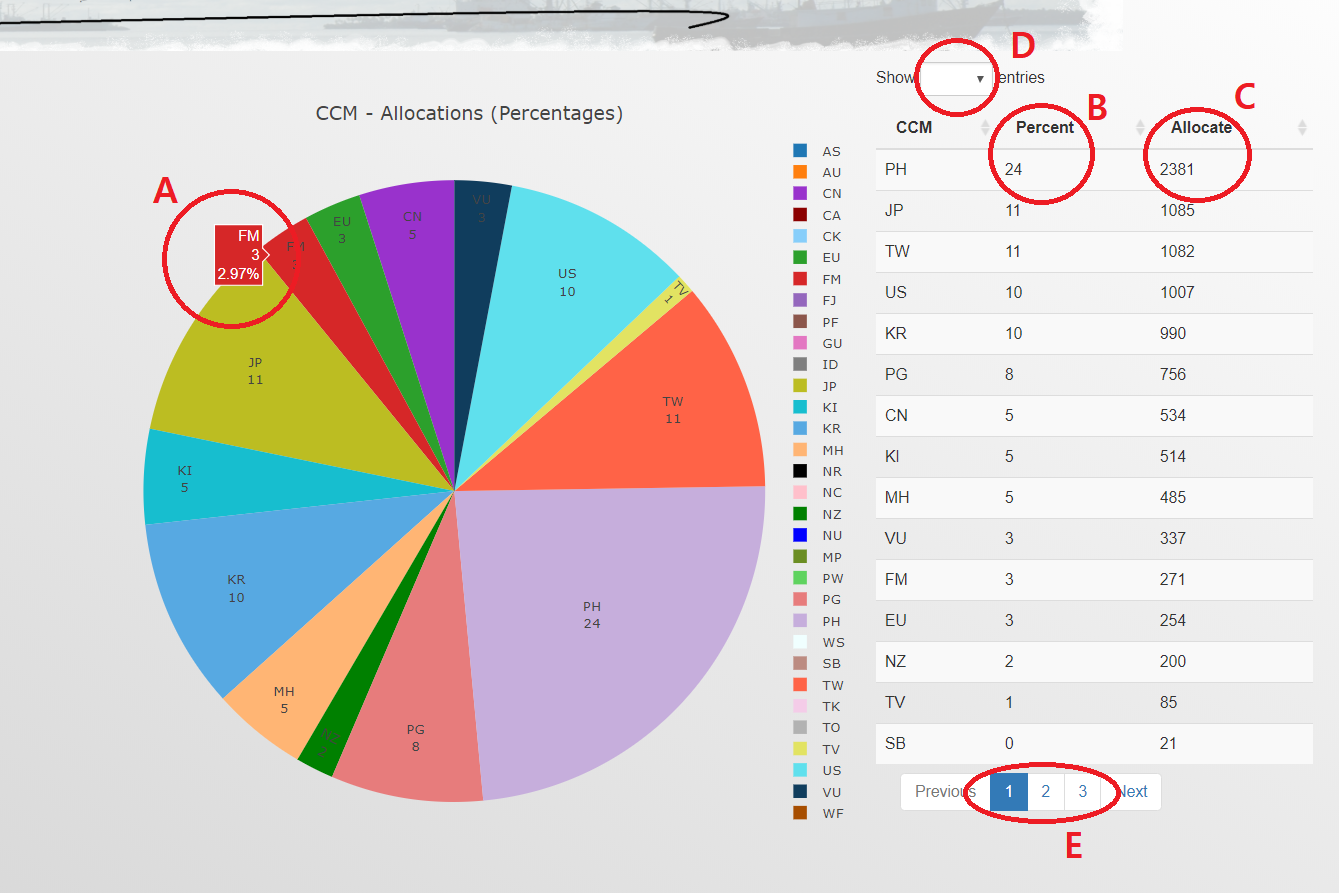
\includegraphics[width=0.95\textwidth]{C:/GitHub/WHATapp/Writing/Output_Figure.png}
  \caption {A picture of part of the app dashboard showing some of the features of the allocation output.}
  \label{fig:outputpic}
\end{figure}


\section{Calculation of values for each criteria} \label{sec:scendet}
This section details the calculations and definitions utilised to determine the values used for each CCM for each criteria. 

\subsection*{Current high seas limits}
\noindent\textbf{\emph{Purse seine:}}
Some CCMs already have purse seine effort limits on the high seas. This criteria uses the values for CCMs that are outlined in table 2 of CMM 2018-01 Attachment 1  (also provided at the end of this document; Fig. \ref{fig:CMM1}) and all CCMs not specified in that table receive zero values. Note that the values for the Philippines are outlined in Attachment 2 of the same document. Also note that the option ``Include HSP1 etc.?'' affects this scenario. If the option ``Exclude pockets'' is chosen then the PH allocation (and only the PH allocation) is excluded, given that their allocation was established to fish in HS pocket I1, which may or may not be relevant for allocating effort on the ``open'' high seas areas.

\noindent\textbf{\emph{Longline:}}
Not available for longline as current limits are flag- rather than zone-based.

\subsection*{Current EEZ limits}
\noindent\textbf{\emph{Purse seine:}}
Many CCMs have purse seine effort limits within their EEZs and these are outlined in table 1 of CMM 2018-01 Attachment 1  (also provided at the end of this document; Fig. \ref{fig:CMM2}). These values are used for all applicable CCMs with the values used for individual PNA members based on the 2019 PAEs which add to a total of {\bf 44,034}. The EEZ limits for Australia, New Caledonia and New Zealand are catch-based and these were converted to effort limits by calculating the mean CPUE for the 3 EEZs and dividing the catch value in the table by the appropriate CPUE to give an equivalent effort-based limit. All CCMs not specified in that table receive a value of zero for this criteria.

\noindent\textbf{\emph{Longline:}}
Not available for longline as current limits are flag- rather than zone-based.

\subsection*{Flag-based catch limits for bigeye}
\noindent\textbf{\emph{Purse seine:}}
Not applicable for purse seine.

\noindent\textbf{\emph{Longline:}}
The CMM 2018-01 outlines flag-based catch limits for bigeye for six countries that include all fishing both within EEZs and in the high seas (also provided at the end of this document; Fig. \ref{fig:CMM3}). The longline limit allocation therefore used these values and all CCMs not specified in that table receive a value of zero for this criteria. {\bf Note - should I transfer the 500 mt from JP to CN before allocation?}

\subsection*{Economic dependency}
{\bf This is up for discussion. Currently I have just put in a placeholder with a 1 if fishing is really important to the countries finances or a 0 if not. Needs work.}

\noindent\textbf{\emph{Purse seine:}}

\noindent\textbf{\emph{Longline:}}

\subsubsection*{Development status}
{\bf This is up for discussion. Currently I have just put in a placeholder with a 1 if the country is a developing country or a 0 if not. Needs work.}

\noindent\textbf{\emph{Purse seine:}}

\subsection*{Biomass of focal stock in EEZs}
\noindent\textbf{\emph{Purse seine:}}

\noindent\textbf{\emph{Longline:}}

\subsection*{EEZ size}
\noindent\textbf{\emph{Purse seine:}}
This was calculated as the area of each EEZ in the WCPFC convention area between 20\degree N and 20\degree S, excluding land area and archipelagic waters. The western boundary of the WCPFC is difficult to define and so we include all waters east of the continental shelf. The Resulting boundaries and EEZs are displayed in Fig. \ref{fig:areaPS}. All CCMs that did not have any part of their EEZ within this region received a value of zero.

\noindent\textbf{\emph{Longline:}}
The same method was used for the longline scenario except that the boundaries were extended into temperate waters with northern and southern boundaries set at {\bf 50\degree N} and {\bf 50\degree S}, respectively (Fig. \ref{fig:areaPS}). EEZ areas are again calculated excluding land and archipelagic waters and all CCMs that did not have any part of their EEZ within this region received a value of zero.

\subsection*{Adjacency}
\noindent\textbf{\emph{Purse seine:}}
Adjacency has been identified as a potentially important allocation scenario. There are several different methods that could be used to quantify what should be considered ``adjacent''. One method calculates the proportion of the high seas area adjacent to each EEZ. This could either be the full high seas areas or only areas within a certain distance (say 100 miles) of an EEZ. The value used for this scenario will then be the relative proportion of adjacent area (of high seas) among each CCM \footnote{Note that we have currently approximated this area by randomly distributing points in the highseas, calculating the closest EEZ and excluding all points further than {\bf 100 nautical miles} from an EEZ (as shown in Fig. \ref{fig:adjPS}). A full GIS buffer measurement approach will be adopted once the parameters have been decided upon.}. This type of calculation therefore benefits CCMs who have long EEZ boundaries shared with the high seas (Fig. \ref{fig:adjPS}). The weakness of this approach is that it gives equal weight to all high seas areas even though the distribution of fish and/or fishing effort is generally very localised.

An alternative approach considers the distribution of fishing effort in the high seas. We can determine the location of all sets from operational logsheet data and determine the nearest EEZ to each set. The value used for the scenario will then be the relative proportion of sets falling nearest to each CCMs EEZ.% Figure {\bf XXXX} shows the distribution of purse seine sets over the period {\bf XXXX--XXXX - I still need to implement this approach}.
\ The weakness of this approach is that logsheet coverage is not perfect and so biases in the distribution of available sets are possible and will affect resulting allocation values, although this is more of a problem for longlining.

\noindent\textbf{\emph{Longline:}}
The approach for longline was identical to described for purse seine except that the areas used were the wider region extending from 50\degree S to 50 \degree N. The longline adjacency figure is shown in Fig. \ref{fig:adjPS}.% The area option and the position of logsheets option are displayed in Fig. \ref{fig:adjPS} and {\bf Fig. - still to implement} , respectively.

\subsection*{Equal split}
Very simply, this criteria allocates over all CCMs equally. This scenario is the same for both purse seine and longline.

\subsection*{Historical effort - purse seine only} \label{sec:histscen}
This criteria allocates more of the TAE to a CCM if it has a history of fishing in the high seas. You have additional choices available in the app for this criteria related to the timing of the calculations of historical effort. Initially, the annual effort fished by each CCM in the high seas between 20\degree N and 20\degree S, for the period 2003--2016 was extracted from the databases. When the tick box for this criteria is checked 3 widgets will appear (see Fig. \ref{fig:HistOp}) - the usual criteria weighting bar ({\bf C} in the figure), but also an additional sliding bar ({\bf A}) and a numeric box ({\bf C}) which together determine the timing and methods of calculating historical effort. Using the year sliding bar you can shift the left and right markers to modify the first and last years of data used for the calculations, respectively. The numerical box can be modified to be one or greater and this determines the number of ``best'' years over which the mean of effort is calculated. For example, if the slider is changed to span 2012--2017 and the numerical box is set to 3, then the mean effort over the 3 highest years of effort fished by each CCM over 2012--2017. Note that the ``weighting'' sliding bar ({C}; Fig. \ref{fig:HistOp}) is identical to those in the other scenarios (e.g. {\bf B} in Fig. \ref{fig:featpg}), and thus it weights the historical scenario against the other scenarios, though only if more than one tickbox is checked of course.

\newpage
 \begin{figure} [h]
  \centering
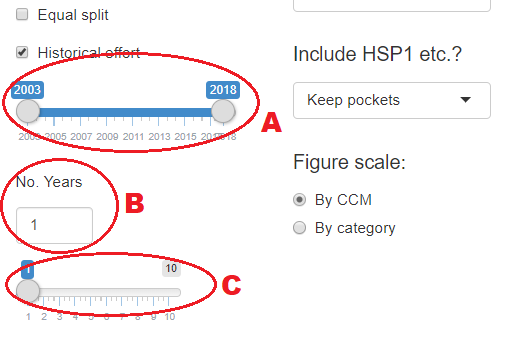
\includegraphics[width=0.6\textwidth]{C:/GitHub/WHATapp/Writing/Historical_Options.png}
  \caption {Screenshot showing the three input widgets that allow the historical effort (catch for longline) scenario to be controlled. These are detailed in section \ref{sec:histscen}.}
  \label{fig:HistOp}
\end{figure}

\subsection*{Historical catch - longline only}
This scenario works in exactly the same manner as the purse seine historical effort scenario except that the metric used is the {\bf total annual catch of target tunas (albacore, bigeye, yellowfin) - IT IS NOT CLEAR TO ME WHAT IS GOING TO BE USED FOR LL - JUST BET???} in the high seas, by each CCM.

\section{A worked example} \label{sec:expl}
We will now examine a specific example to clarify the features available and the interpretation of the output. We will examine a purse seine scenario where more than one scenario is used to allocate a total allowable effort on the high seas. The steps to follow are outlined below and the setting are displayed in Fig. \ref{fig:explapp}:
\begin{enumerate}
\item Select purse seine under the gear type selector ({\it A} in Fig. \ref{fig:explapp}).
\item Type in a total allowable effort of 15,000 days ({\it B}).
\item ``Include PH'' in the appropriate selector ({\it C}).
\item ``Exclude pockets'' in the appropriate selector ({\it D}).
\item Ensure that ``By CCM'' is selected under ``Figure scale'' ({\it E}).
\item Now move to the scenarios options column (on the left) and click scenarios ``Development status'' and ``Adjacency'' ({\it F's}).
\item Now click on the ``Historical effort'' scenario and shift the left dot on the sliding bar to 2014 while keeping the right dot on 2018 ({\it G}). Type ``5'' into the ``No. Years'' box ({\it H}).
\item Now we can weight the 3 selected scenarios. Keep the sliding bar for development status on 1, move the sliding bar for adjacency to 2 and to 4 for the historical effort ({\it I}). Watch how this affects the allocations as you change the weightings.
\end{enumerate}
We are now ready to examine the results of this potential allocation scenario. A few points must be addressed first however. This scenario starts by deciding that there will be 15,000 days of purse seine effort in the high seas and this total will be allocated amongst CCMs based on the 3 selected scenarios. The historical effort scenarios is set up so that only the last 5 years are considered (2014--2018), and the value calculated is the mean effort fished by each CCM over those 5 years. The 3 scenarios are then given weights and the values chosen mean that we are assuming the the adjacency scenario will have twice the influence of development status, and historical effort will have 4 times the influence of development status (and twice the influence of adjacency).

The pie chart and the table show the results of using a scenario such as this, with the higest number of days being allocated to {\bf XX (XX\%; XX days), XX (XX\%; XX days) and XX (XX\%; XX days)}. You should be able to find how many days would be allocated to your individual country by looking in the table (scroll through the ``pages'' if it is not on the first page). If you now select ``By category'' under the ``Figure scale'' option  ({\it J}) you will be able to see how the TAE would be allocated amongst the sub regional categories.

 \begin{figure}[h]
  \centering
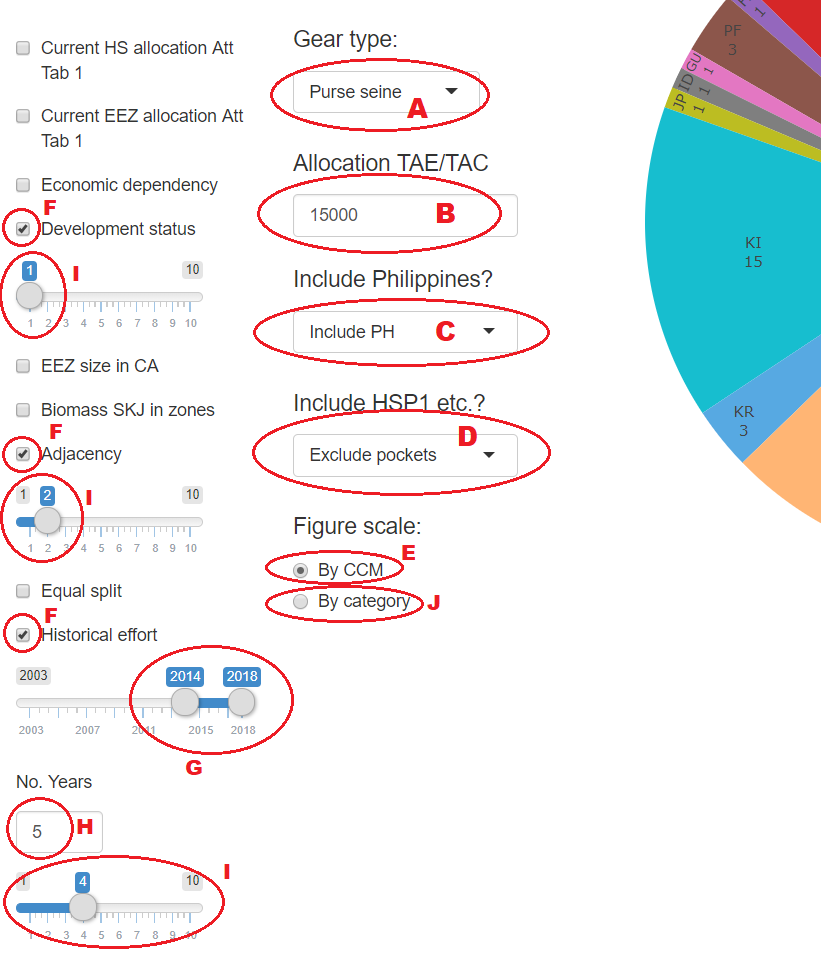
\includegraphics[width=0.8\textwidth]{C:/GitHub/WHATapp/Writing/Worked_Example.png}
  \caption {Screenshot of the app showing the settings outlined in the worked example in section \ref{sec:expl}.}
  \label{fig:explapp}
\end{figure}


\section{General discussion}
The purpose of the software and this report is to make the visualisation of potential allocation scenarios easily accessible to members. To this end we welcome feedback on how the app could be improved. This may include improvements in the presentation of results or the instructions of how the app is to be used. It should also be noted that this tool is a work in progress and only reflects the discussions regarding allocations that have taken place so far. As further scenarios are proposed or existing ones are modified, then these will be added to the tool.

\clearpage

 \begin{figure}[!htb]
 \centering

   \subfloat{%
    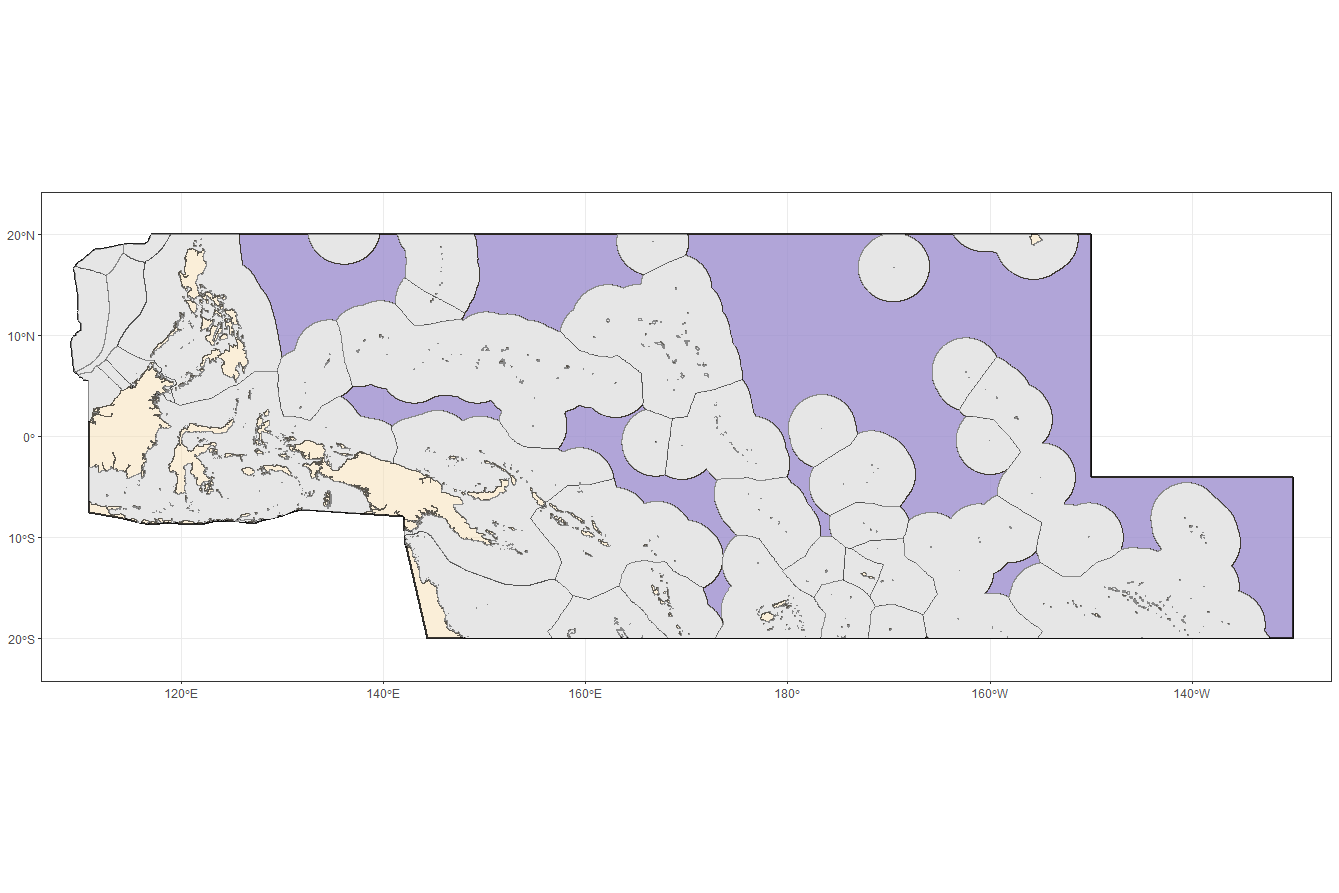
\includegraphics[width=0.9\textwidth]{C:/GitHub/WHATapp/EEZs/Plots/HSareas_20-20_Areas.png}}
   \subfloat{%
    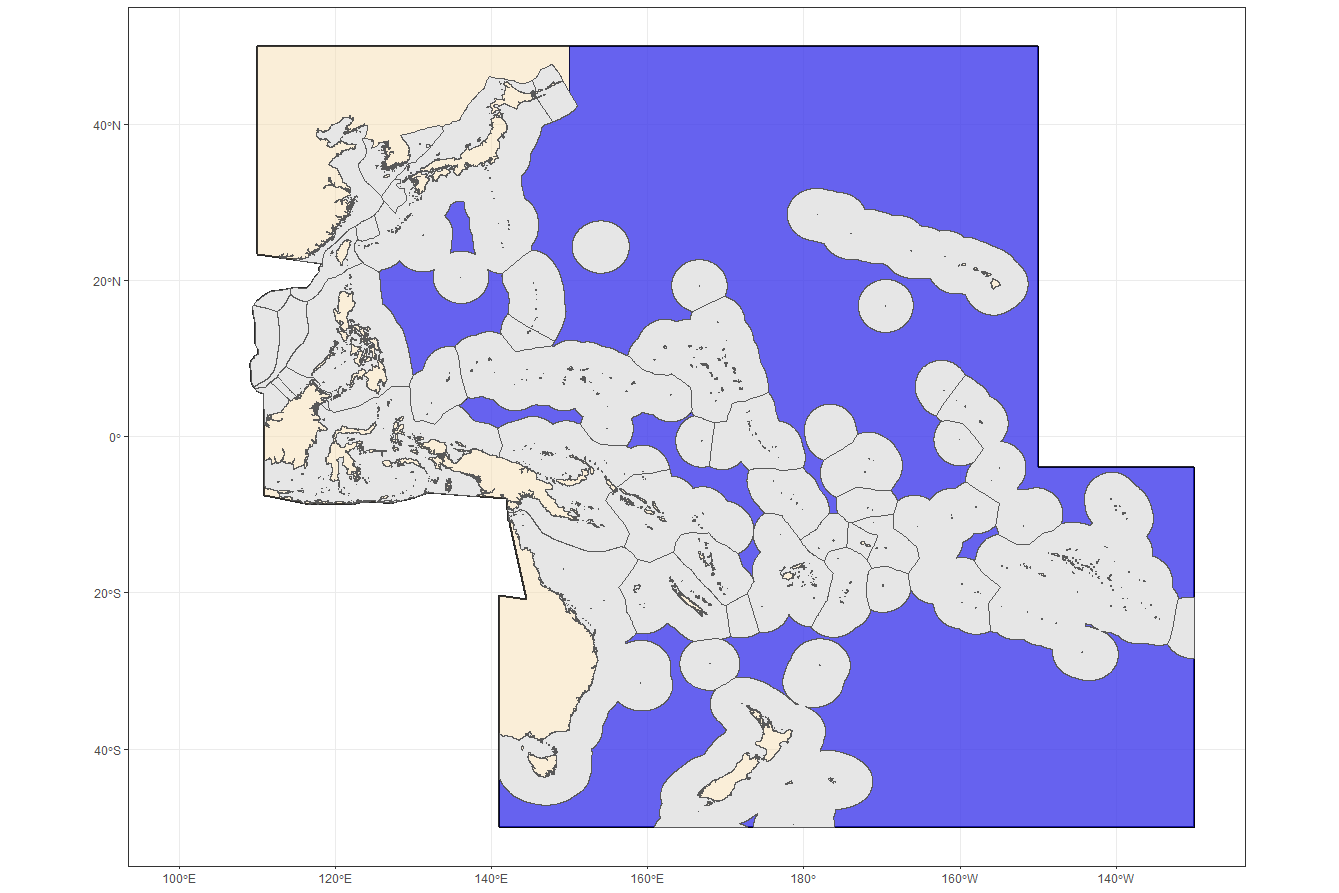
\includegraphics[width=0.9\textwidth]{C:/GitHub/WHATapp/EEZs/Plots/HSareas_LL_Areas_JustHS.png}} \\
 \caption{Maps showing the high seas areas (purple) relevant for the purse seine (top) and longline (bottom) scenarios.}\label{fig:HSareasPS}
 \end{figure}


 \begin{figure}[!htb]
 \centering

   \subfloat{%
    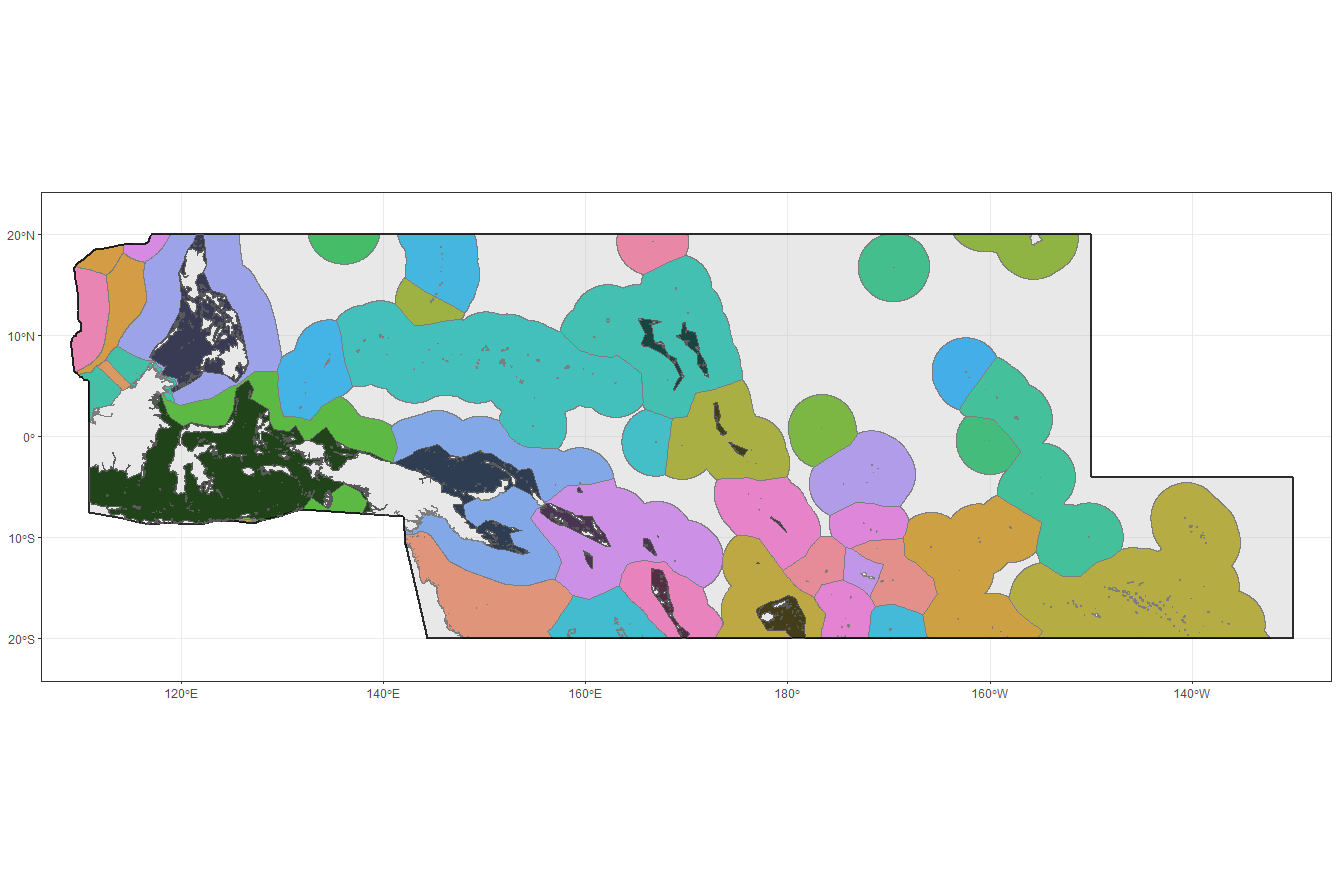
\includegraphics[width=0.9\textwidth]{C:/GitHub/WHATapp/EEZs/Plots/EEZareas_20-20_Areas-Arch_NoOverlap.png}}
   \subfloat{%
    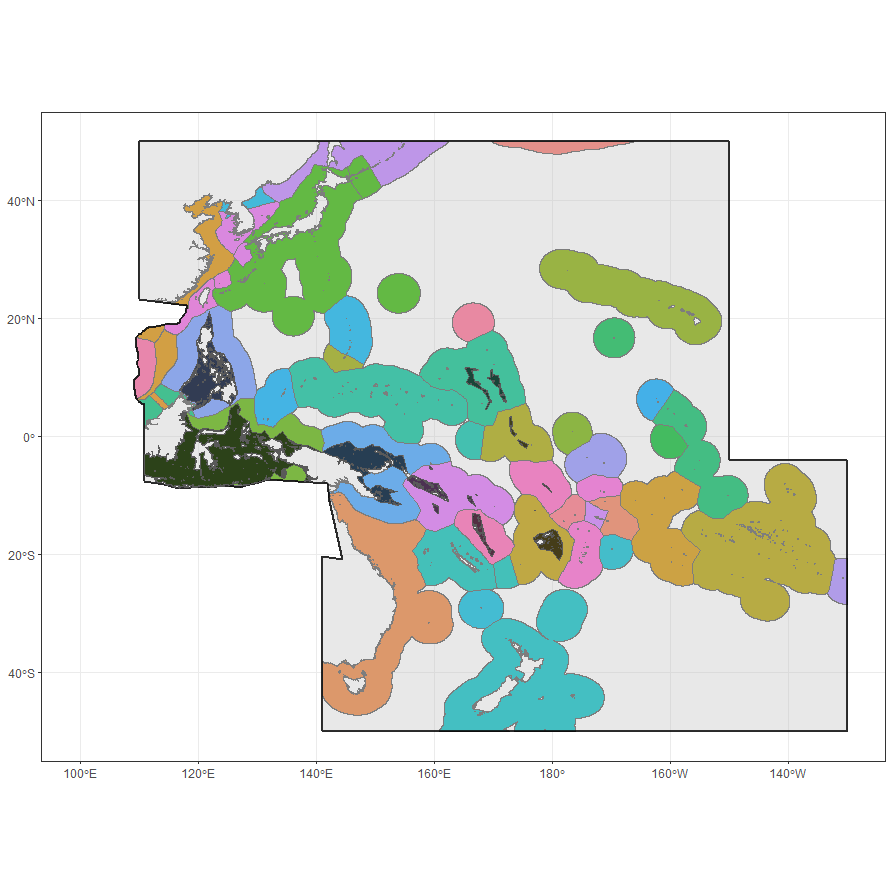
\includegraphics[width=0.9\textwidth]{C:/GitHub/WHATapp/EEZs/Plots/EEZareas_LL_Areas-Arch_NoOverlap.png}} \\
 \caption{Maps showing the EEZ areas within the purse seine (top) and longline (bottom) scenario zones. Archepelagic waters are shown as black shaded areas.}\label{fig:areaPS}
 \end{figure}


 \begin{figure}[!htb]
 \centering

   \subfloat{%
    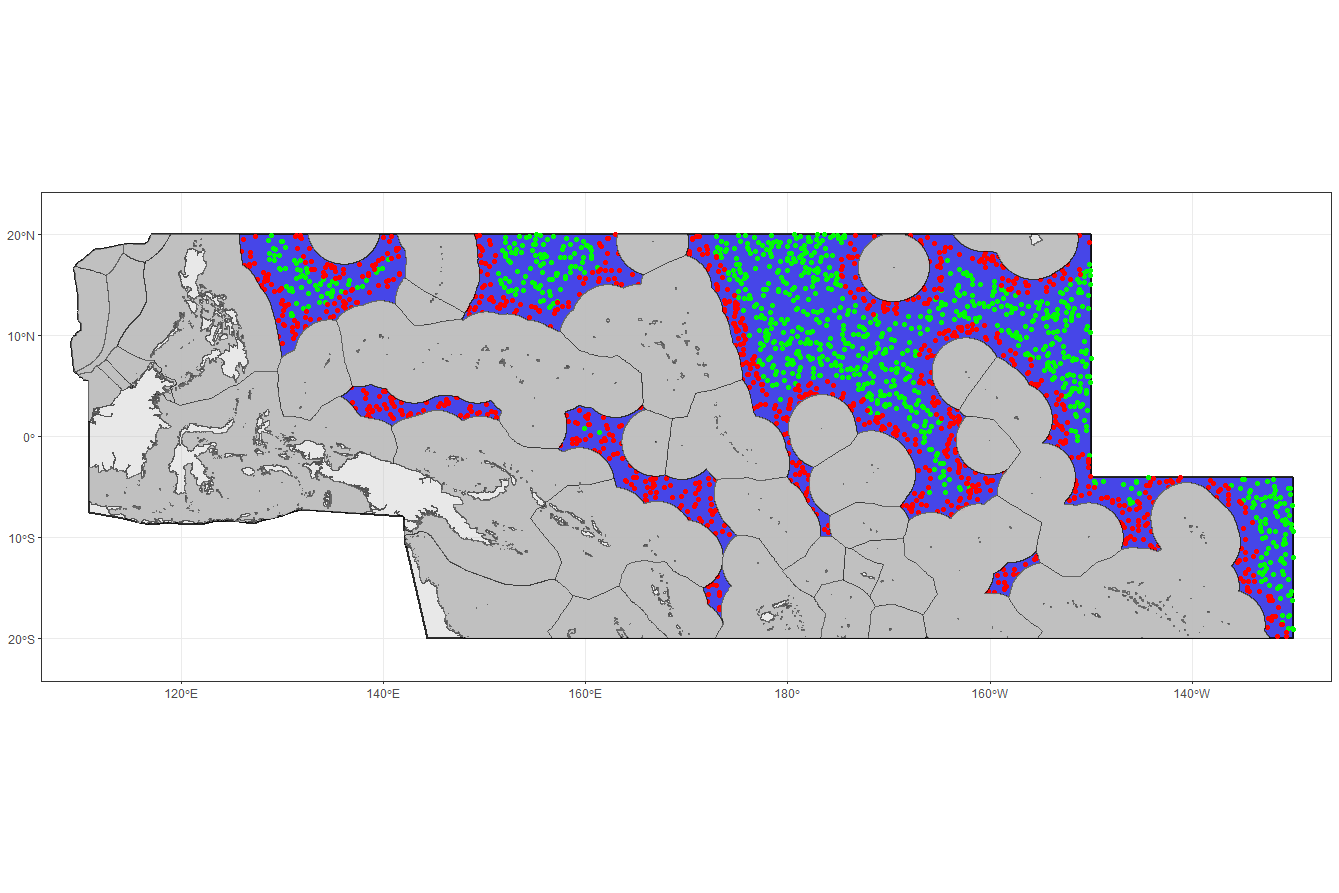
\includegraphics[width=0.9\textwidth]{C:/GitHub/WHATapp/EEZs/Plots/HSareas_20-20_Areas_AllPnts-In-Out_Close.png}}
   \subfloat{%
    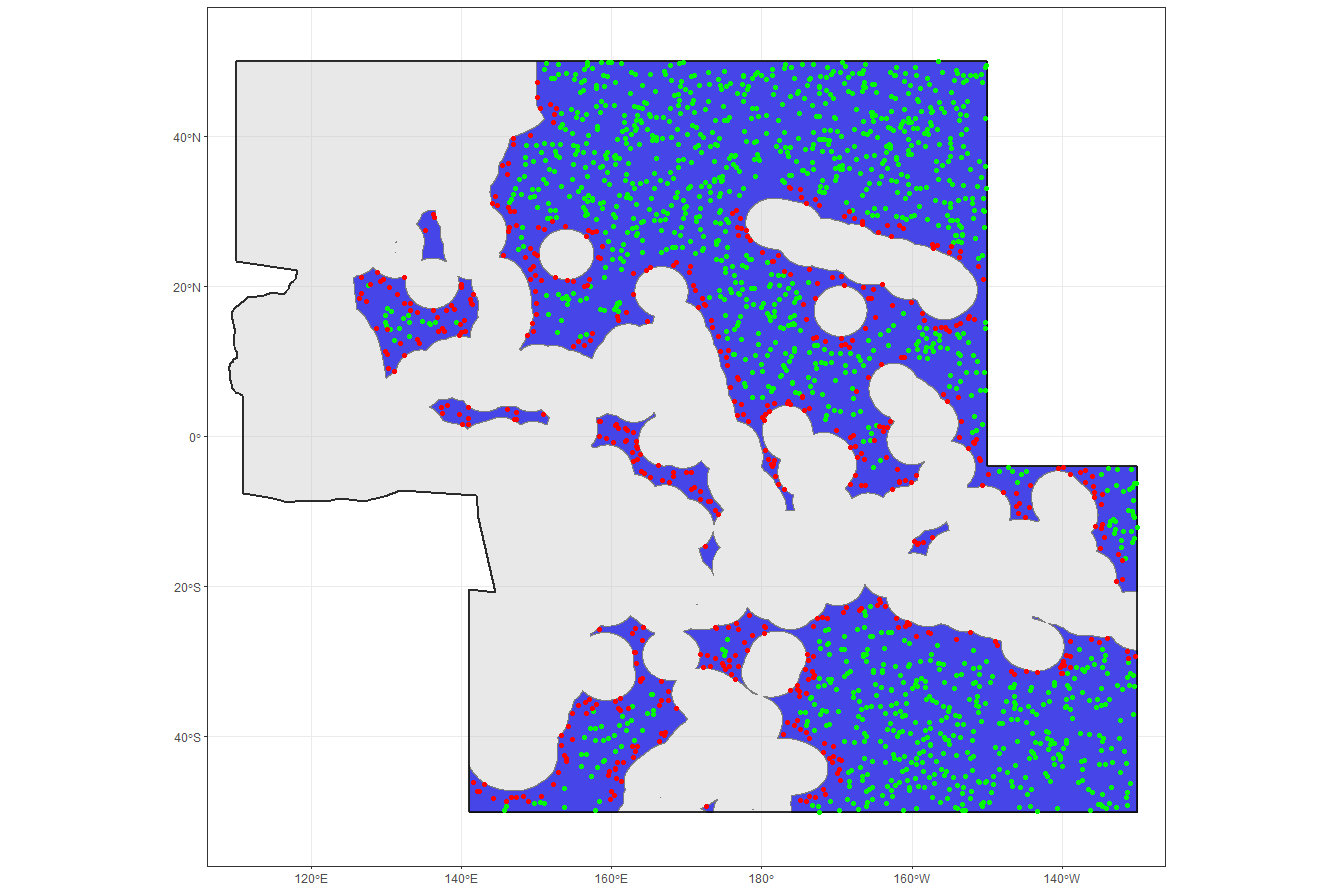
\includegraphics[width=0.9\textwidth]{C:/GitHub/WHATapp/EEZs/Plots/HSareas_Longline_Areas_AllPnts-In-Out_Close.png}} \\
 \caption{Maps showing the locations of random points distributed in high seas areas for the purse seine (top) and longline (bottom) scenarios. Red points are within 100 nautical miles of an EEZ and the closest EEZ to each point is measured to calculate relative allocations. Green points are greater than 100 miles from any EEZ and are discarded.}\label{fig:adjPS}
 \end{figure}


\newpage
 \begin{figure}[!htb]
  \centering
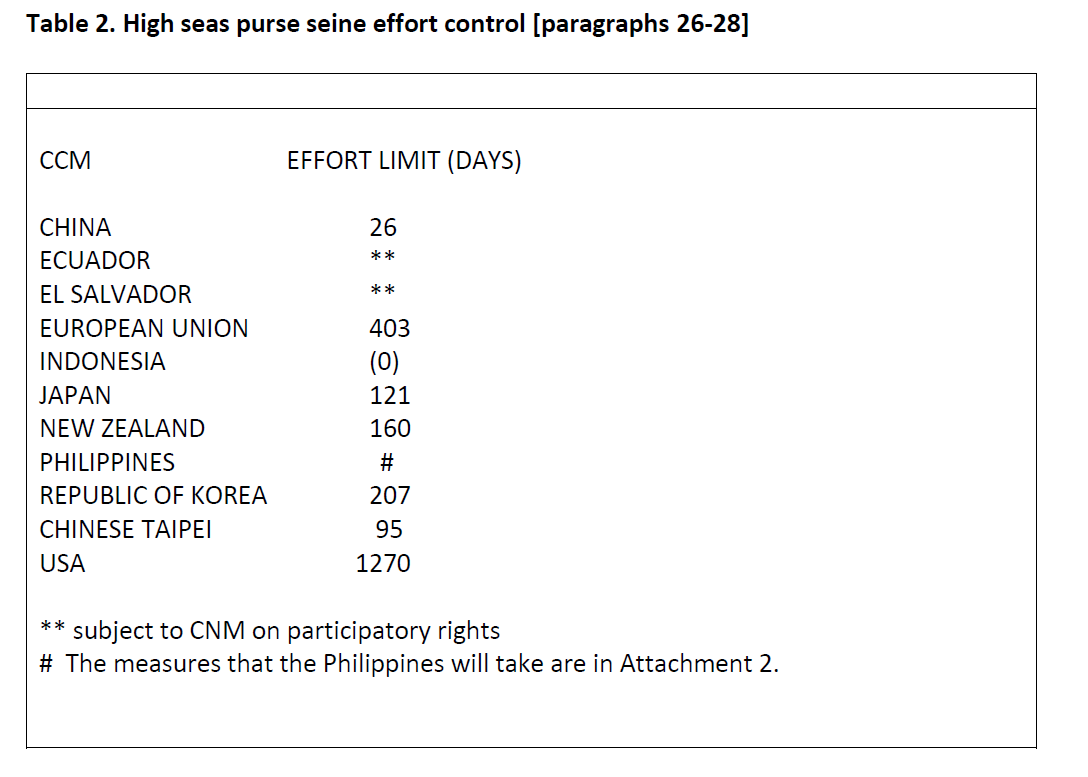
\includegraphics[width=1\textwidth]{C:/GitHub/WHATapp/Writing/CMM_PS_HS_Limits.png}
  \caption {Effort limits for various flags in the high seas as specified in the appendix of CMM 2018-01.}
  \label{fig:CMM1}
\end{figure}


\newpage
 \begin{figure}[!htb]
  \centering
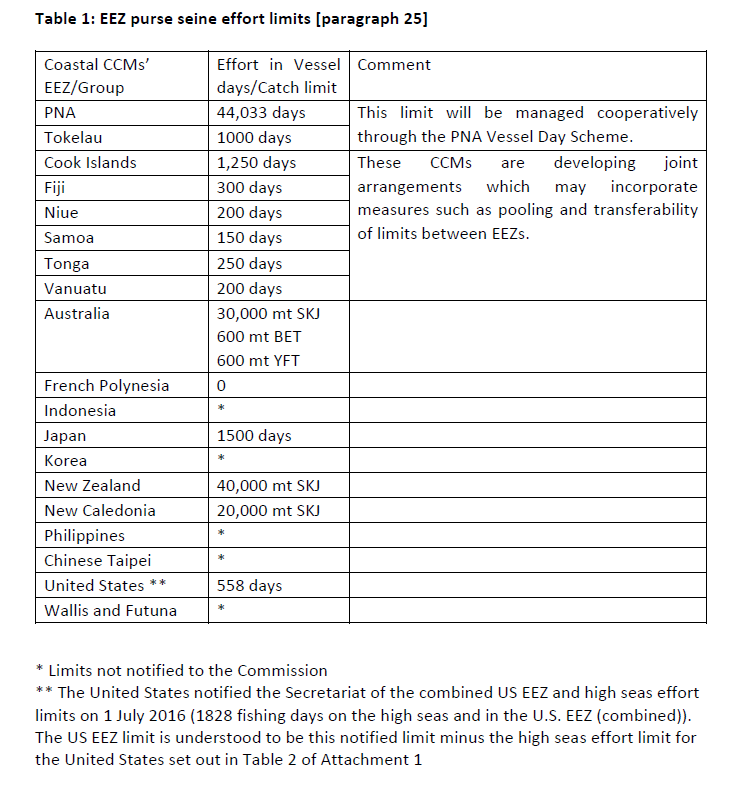
\includegraphics[width=1\textwidth]{C:/GitHub/WHATapp/Writing/CMM_PS_EEZ_Limits.png}
  \caption {Effort limits for various EEZs in the WCPO as specified in the appendix of CMM 2018-01.}
  \label{fig:CMM2}
\end{figure}


\newpage
 \begin{figure}[!htb]
  \centering
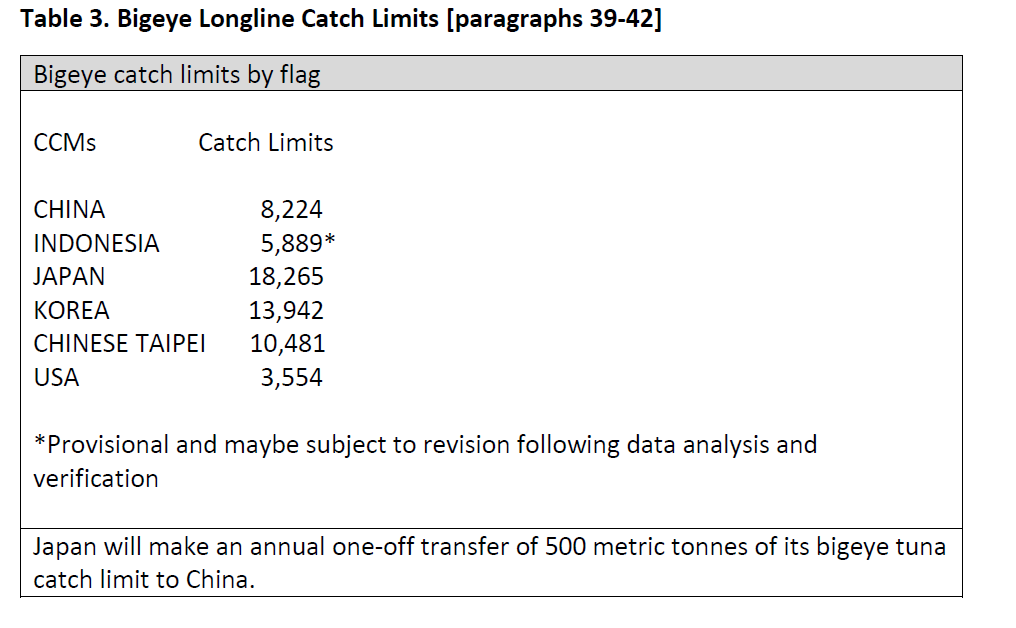
\includegraphics[width=1\textwidth]{C:/GitHub/WHATapp/Writing/CMM_Bigeye_Flag_Limits.png}
  \caption {Flag-based catch limits for bigeye tuna as specified in the appendix of CMM 2018-01.}
  \label{fig:CMM3}
\end{figure}


\end{document}
